\section{StartupBench 任务标注教程}

\subsection{任务构建}
\label{app:task_construction}

一项 \textsc{startup} 任务可定义为三元组 $\mathcal{T}=(q,\mathcal{E},\mathcal{R})$。专家必须提供任务的全部要素：

\begin{itemize}
    \item \textbf{输入请求：}请求 $q$ 是对任务的自然语言表述，规定启动任务的用户指令。输入请求源自标注者工作的真实场景，应反映现实用户意图，包括任务背景、隐含约束和预期交付物。

    \item \textbf{任务工作空间：}环境 $\mathcal{E}$ 表示提供给智能体的完整工作空间，包括多模态源文件，以及完成任务所需的其他资源和交互设置。任务工作空间为智能体提供自包含的执行环境。每个工作空间都包含完成任务所需的全部输入产物（例如文件、数据集或结构化资源），并确保智能体能够获得足够的输入信息来解决问题。该设计既能在受控条件下进行可复现评估，也保留了现实工作流结构。

    \item \textbf{评估细则：}评分细则 $\mathcal{R}=\{(p_i,w_i)\}_{i=1}^{n}$ 是一张核对表，其中每一项都包含自然语言评分点 $p_i$ 和正的重要性权重 $w_i$；权重反映该项对成功完成任务的重要程度。评估细则定义了一组用于考查任务完成质量的细粒度标准。由于现实工作流复杂且涉及多个方面，每项任务均使用覆盖不同维度的多条评分细则进行评估。我们把 StartupBench 的全部评分细则分为 6 个维度和 3 个重要性层级，详见附录~\ref{app:rubrics}。
\end{itemize}

这些组成部分共同保留了现实智能体工作流的结构，同时支持系统、客观的评估。任务可能要求信息综合、约束遵循、结构化生成，或领域特定的推理与判断。

\subsection{交叉验证}
\label{app:cross_valid}

为保证数据质量的可靠性，在构建过程中，每项任务至少由另一位具有相关专业经验的领域专家独立审查。审查者并非只关注标注一致性，而是从多个互补视角验证任务的真实性和正确性。

\begin{itemize}
\item \textbf{任务真实性。}审查者核验任务描述和配套工作空间的真实性，包括检查输入请求是否反映现实用户要求、全部所给材料是否事实正确，以及是否不存在领域知识错误。

\item \textbf{工作流忠实度。}审查者考查任务是否忠实代表相应职业中的现实工作流。偏离实际工作程序或不能反映真实岗位职责的任务会被修订或舍弃。

\item \textbf{评分细则有效性。}审查者检查评估细则，确保被考查能力对目标工作流有意义、各条细则清晰且无歧义，其相对权重也能合理反映任务优先级。

\item \textbf{真实答案验证。}审查者使用最终评分细则评估参考解答（真实答案），以验证该解答。真实答案交付物必须取得满分。如果发现参考解答与评估标准不一致，则同时修订解答和评分细则，直至二者相互一致。
\end{itemize}

\section{领域专家背景}
\label{app:expert background}
我们招募了 57 位领域专家，支持任务构建和交叉验证。专家团队覆盖 StartupBench 全部 6 个领域，并拥有多样的专业背景，包括临床医学、法律、投资与量化金融、软件开发与人工智能、工程、商业管理与咨询，以及教育与人文学科。我们根据专家报告的专长领域和职业经验分配任务，以确保任务构建和审查由熟悉相应专业领域的人员完成。

表~\ref{tab:expert_background} 汇总了专家团队的职业经验。其中位职业经验为 5 年。在 57 位专家中，68.4\% 拥有至少 3 年职业经验，42.1\% 拥有至少 6 年职业经验，24.6\% 拥有至少 10 年职业经验。这些背景为把访谈得到的用户场景转化为可复现基准任务，以及在交叉验证期间评估任务的真实性、正确性和评估标准，提供了实践领域知识。所有专家均根据任务构建和审查的实际工作量获得合理报酬。

\begin{table}[t]
\centering
\small
\caption{领域专家背景汇总。职业经验指受访者报告的、在相应或密切相关领域中的经验年数。}
\label{tab:expert_background}
\begin{tabular}{lc}
\toprule
\textbf{专家统计} & \textbf{数值} \\
\midrule
领域专家人数 & 57 \\
职业经验中位数 & 5 年 \\
职业经验 $\geq 3$ 年的专家 & 68.4\% \\
职业经验 $\geq 6$ 年的专家 & 42.1\% \\
职业经验 $\geq 10$ 年的专家 & 24.6\% \\
StartupBench 领域覆盖 & 6 / 6 \\
\bottomrule
\end{tabular}
\end{table}

\section{StartupBench 评分细则}
\label{app:rubrics}

\textbf{评分细则维度。}为在异构现实任务之间实现一致评估，我们按照主要考查能力，把全部评估细则组织为六个高层类别。这些类别并不绑定特定应用领域，而是刻画办公任务中反复出现的交付物质量共性维度，包括正确性、完整性、数据处理、专业推理、工程质量和呈现质量。这套分类既维持了跨任务类型的统一评估框架，又能使模型优缺点分析更易解释。

\begin{itemize}
    \item \textbf{结构与完整性。}评估是否按照正确组织、文件结构和必需组成部分，完整生成了要求的交付物，以及其总体完整程度。

    \item \textbf{计算精度。}评估数值结果、逻辑推理、公式执行、事实一致性和其他客观计算的正确性。

    \item \textbf{信息整合。}评估数据清洗、变换、聚合、统计分析、特征工程、建模和其他结构化数据处理工作流。

    \item \textbf{领域特定合规性。}评估输出是否满足领域特定的专业要求，包括业务逻辑、金融原则、法律推理、医疗实践、教育标准和其他专家知识。

    \item \textbf{工程与格式。}评估实现质量、编码规范、电子表格工程、文档格式、可复现性、稳健性、命名规范，以及对技术规格的遵守情况。

    \item \textbf{输出与呈现。}评估视觉呈现和沟通质量，包括图表、布局、格式、可读性、报告组织，以及最终交付物的总体可用性。
\end{itemize}

表~\ref{tab:rubric_distribution} 汇总了 StartupBench 全部 2,453 条评分细则的分布。计算精度是最大的细则类别，占 38.9\%，反映了生成客观正确的工作成果的重要性。结构与完整性和领域特定合规性合计再占 42.8\%，表明要成功完成现实办公工作流，不仅需要正确计算，还需要完整的交付物和专业领域推理。

\begin{table}[h]
\centering
\small
\caption{StartupBench 评分细则类别分布。}
\label{tab:rubric_distribution}
\begin{tabular}{lc}
\toprule
\textbf{类别} & \textbf{占比} \\
\midrule
结构与完整性 & 27.31\% \\
计算精度 & 38.89\% \\
信息整合 & 9.46\% \\
领域特定合规性 & 15.49\% \\
工程与格式 & 6.20\% \\
输出与呈现 & 2.65\% \\
\midrule
\textbf{总计} & \textbf{100.00\%} \\
\bottomrule
\end{tabular}
\end{table}

\textbf{评分细则重要性层级。}为体现不同要求对成功完成任务的重要程度差异，我们把每条评分细则划分到三个重要性层级之一。\textbf{核心}细则刻画直接决定主要用户需求是否得到满足的要求；违反这些要求会严重损害最终交付物的正确性、可靠性、安全性或可用性。\textbf{重要}细则代表高质量完成任务的关键要求，满足与否会实质影响交付物总体质量，但单独违反其中一条不一定导致交付物不可用。\textbf{辅助}细则刻画层级较低的要求；遗漏它们主要影响细节、用户体验、视觉吸引力或精致程度，而不是交付物的基本可用性。我们分别为核心、重要和辅助细则赋予 \textbf{5}、\textbf{3} 和 \textbf{1} 的权重，并在把细则级判断聚合为任务分数时使用这些权重。图~\ref{fig:rubric_level} 展示了一个含不同层级评分细则的典型任务案例。

\begin{figure*}[t]
    \centering
    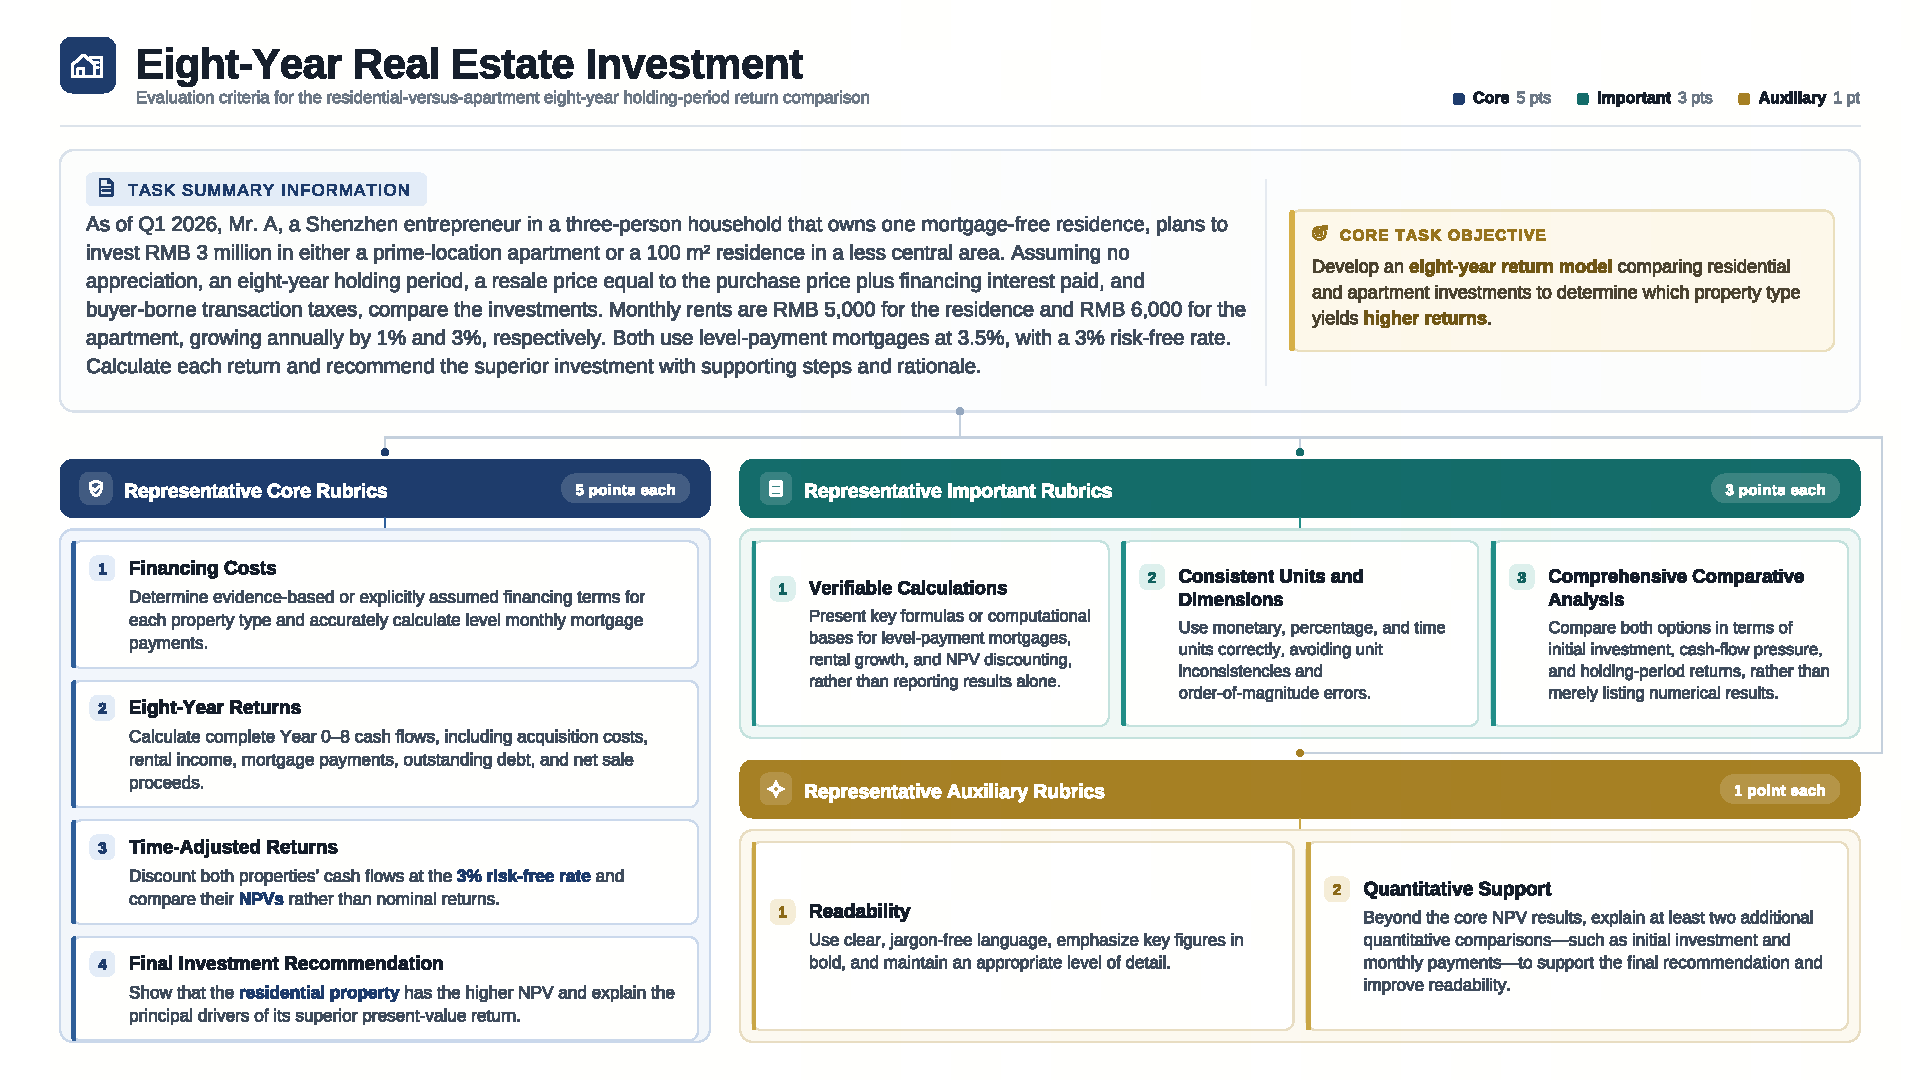
\includegraphics[width=0.99\textwidth]{figures/multi_level_rubric.pdf}
    \caption{一项任务中跨越三个层级的评分细则代表性示例。核心细则考查解决投资问题所必需的金融推理和计算；重要细则评估辅助分析的正确性与完整性；辅助细则则关注呈现质量和额外的定量支持。}
    \label{fig:rubric_level}
\end{figure*}

在所有任务中，核心、重要和辅助细则的权重占比平均分别为 59.10\%、34.33\% 和 6.57\%，从而确保任务分数主要由会实质影响任务成功完成的要求决定。

\section{行为层面失败模式示例}

\subsection{自我验证幻觉}
\label{app:self-verify hallucination}

图~\ref{fig:self_verify} 展示了一个代表性案例。任务要求模型筛选出所有 11 级成员，模拟路线签到直至每位成员达到 12 级阈值，并生成满足一组精确数值和格式约束的 Excel 工作簿。生成的工作簿看似大体完整，包含所需工作表、成员记录和输出列，因而模型断定任务已经成功完成。然而，产物层面检查发现了多项会影响验收的关键错误，包括有效点数数值不正确以及成员姓名不匹配。根本问题并非模型不能执行要求的计算，而是它从未核验自己生成的产物。模型反而把成功的执行摘要当成最终交付物已经得到验证的证据。于是，局部却对用户至关重要的错误未被发现，体现出一种\emph{自我验证幻觉}：模型的信心来自推理过程，而不是根据原始任务要求独立检查已完成的产物。

\begin{figure*}[t]
    \centering
    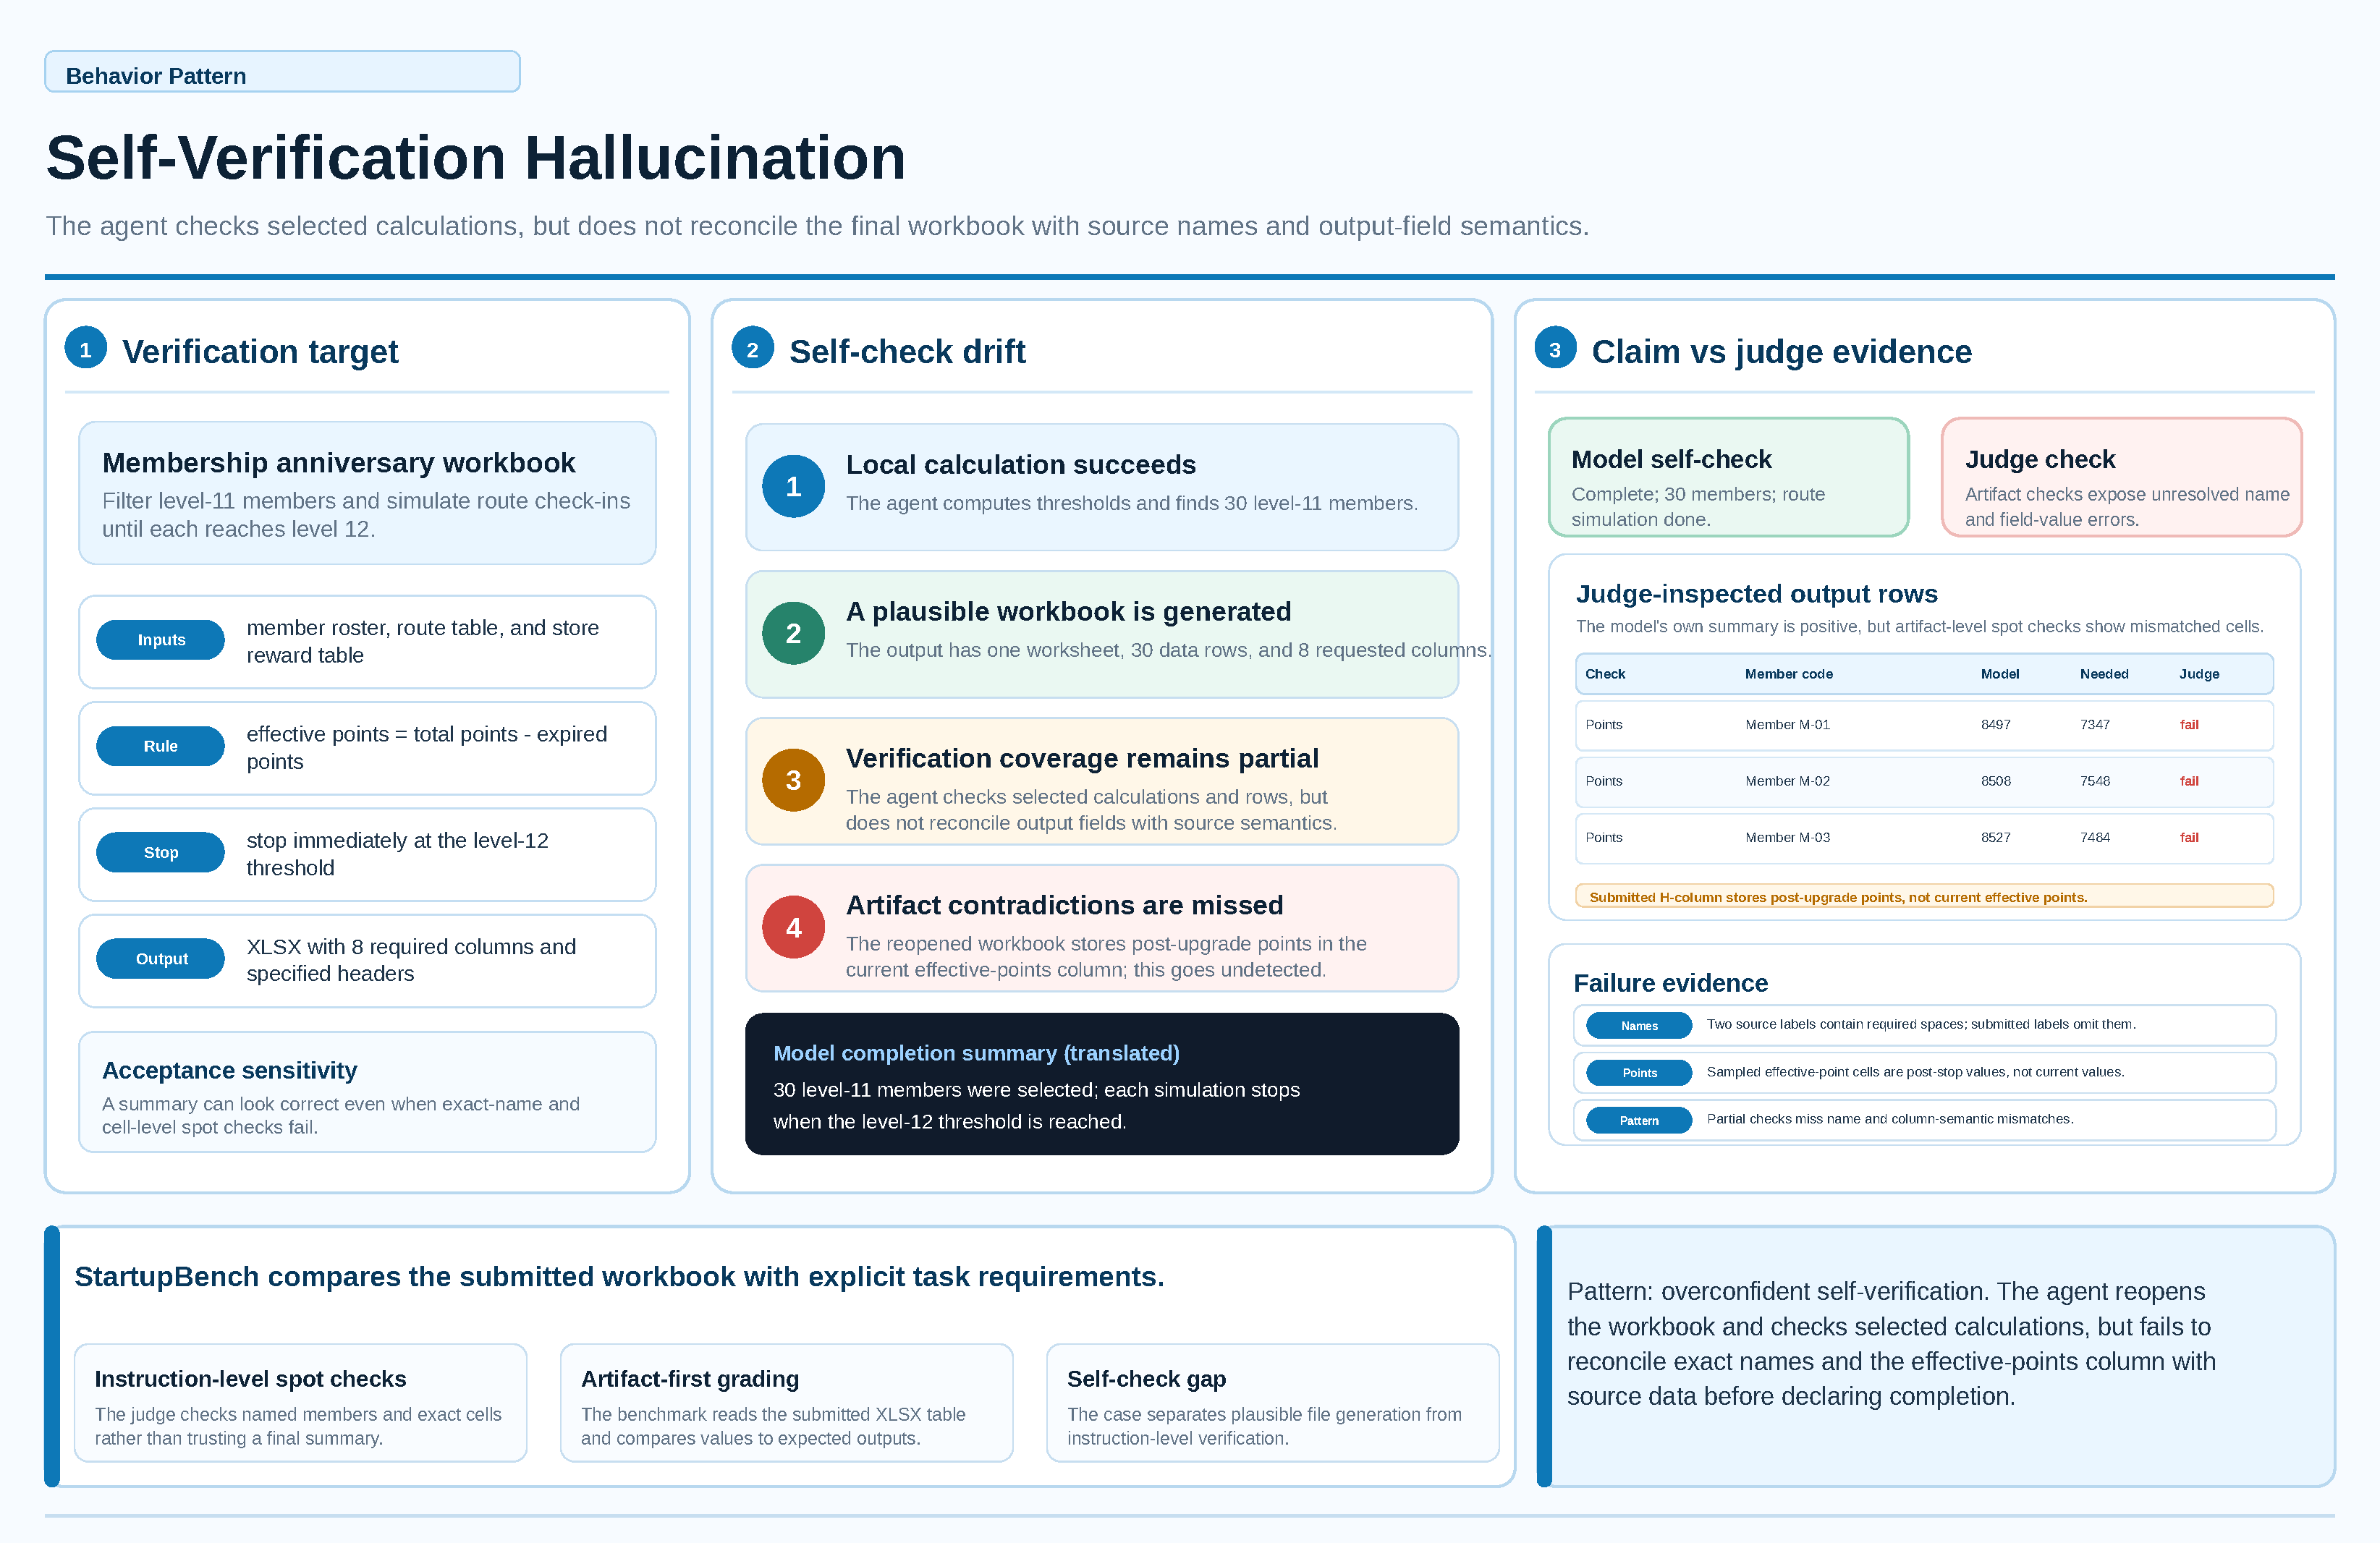
\includegraphics[width=0.99\textwidth]{figures/figure6_self_verification_hallucination.pdf}
    \caption{自我验证幻觉的代表性示例。模型生成了一个看似合理的工作簿，并根据执行过程断定任务已经完成；但产物层面的抽查揭示出最终交付物中影响验收的关键错误，表明模型把进度摘要误作真正的验证，没有根据原始任务要求核验生成的产物。}
    \label{fig:self_verify}
\end{figure*}

\subsection{领域特定失败}
\label{app:domain}

图~\ref{fig:domain-specify} 展示了一个由领域特定临床可操作性不足导致的代表性失败案例。模型生成了一份格式良好、看似符合临床专业标准的多学科治疗计划，却违反了多项安全关键型治疗约束。该失败并非源于写作质量不佳，而是源于模型无法把医学知识转化为可操作且临床可靠的决策。

\begin{figure*}[t]
    \centering
    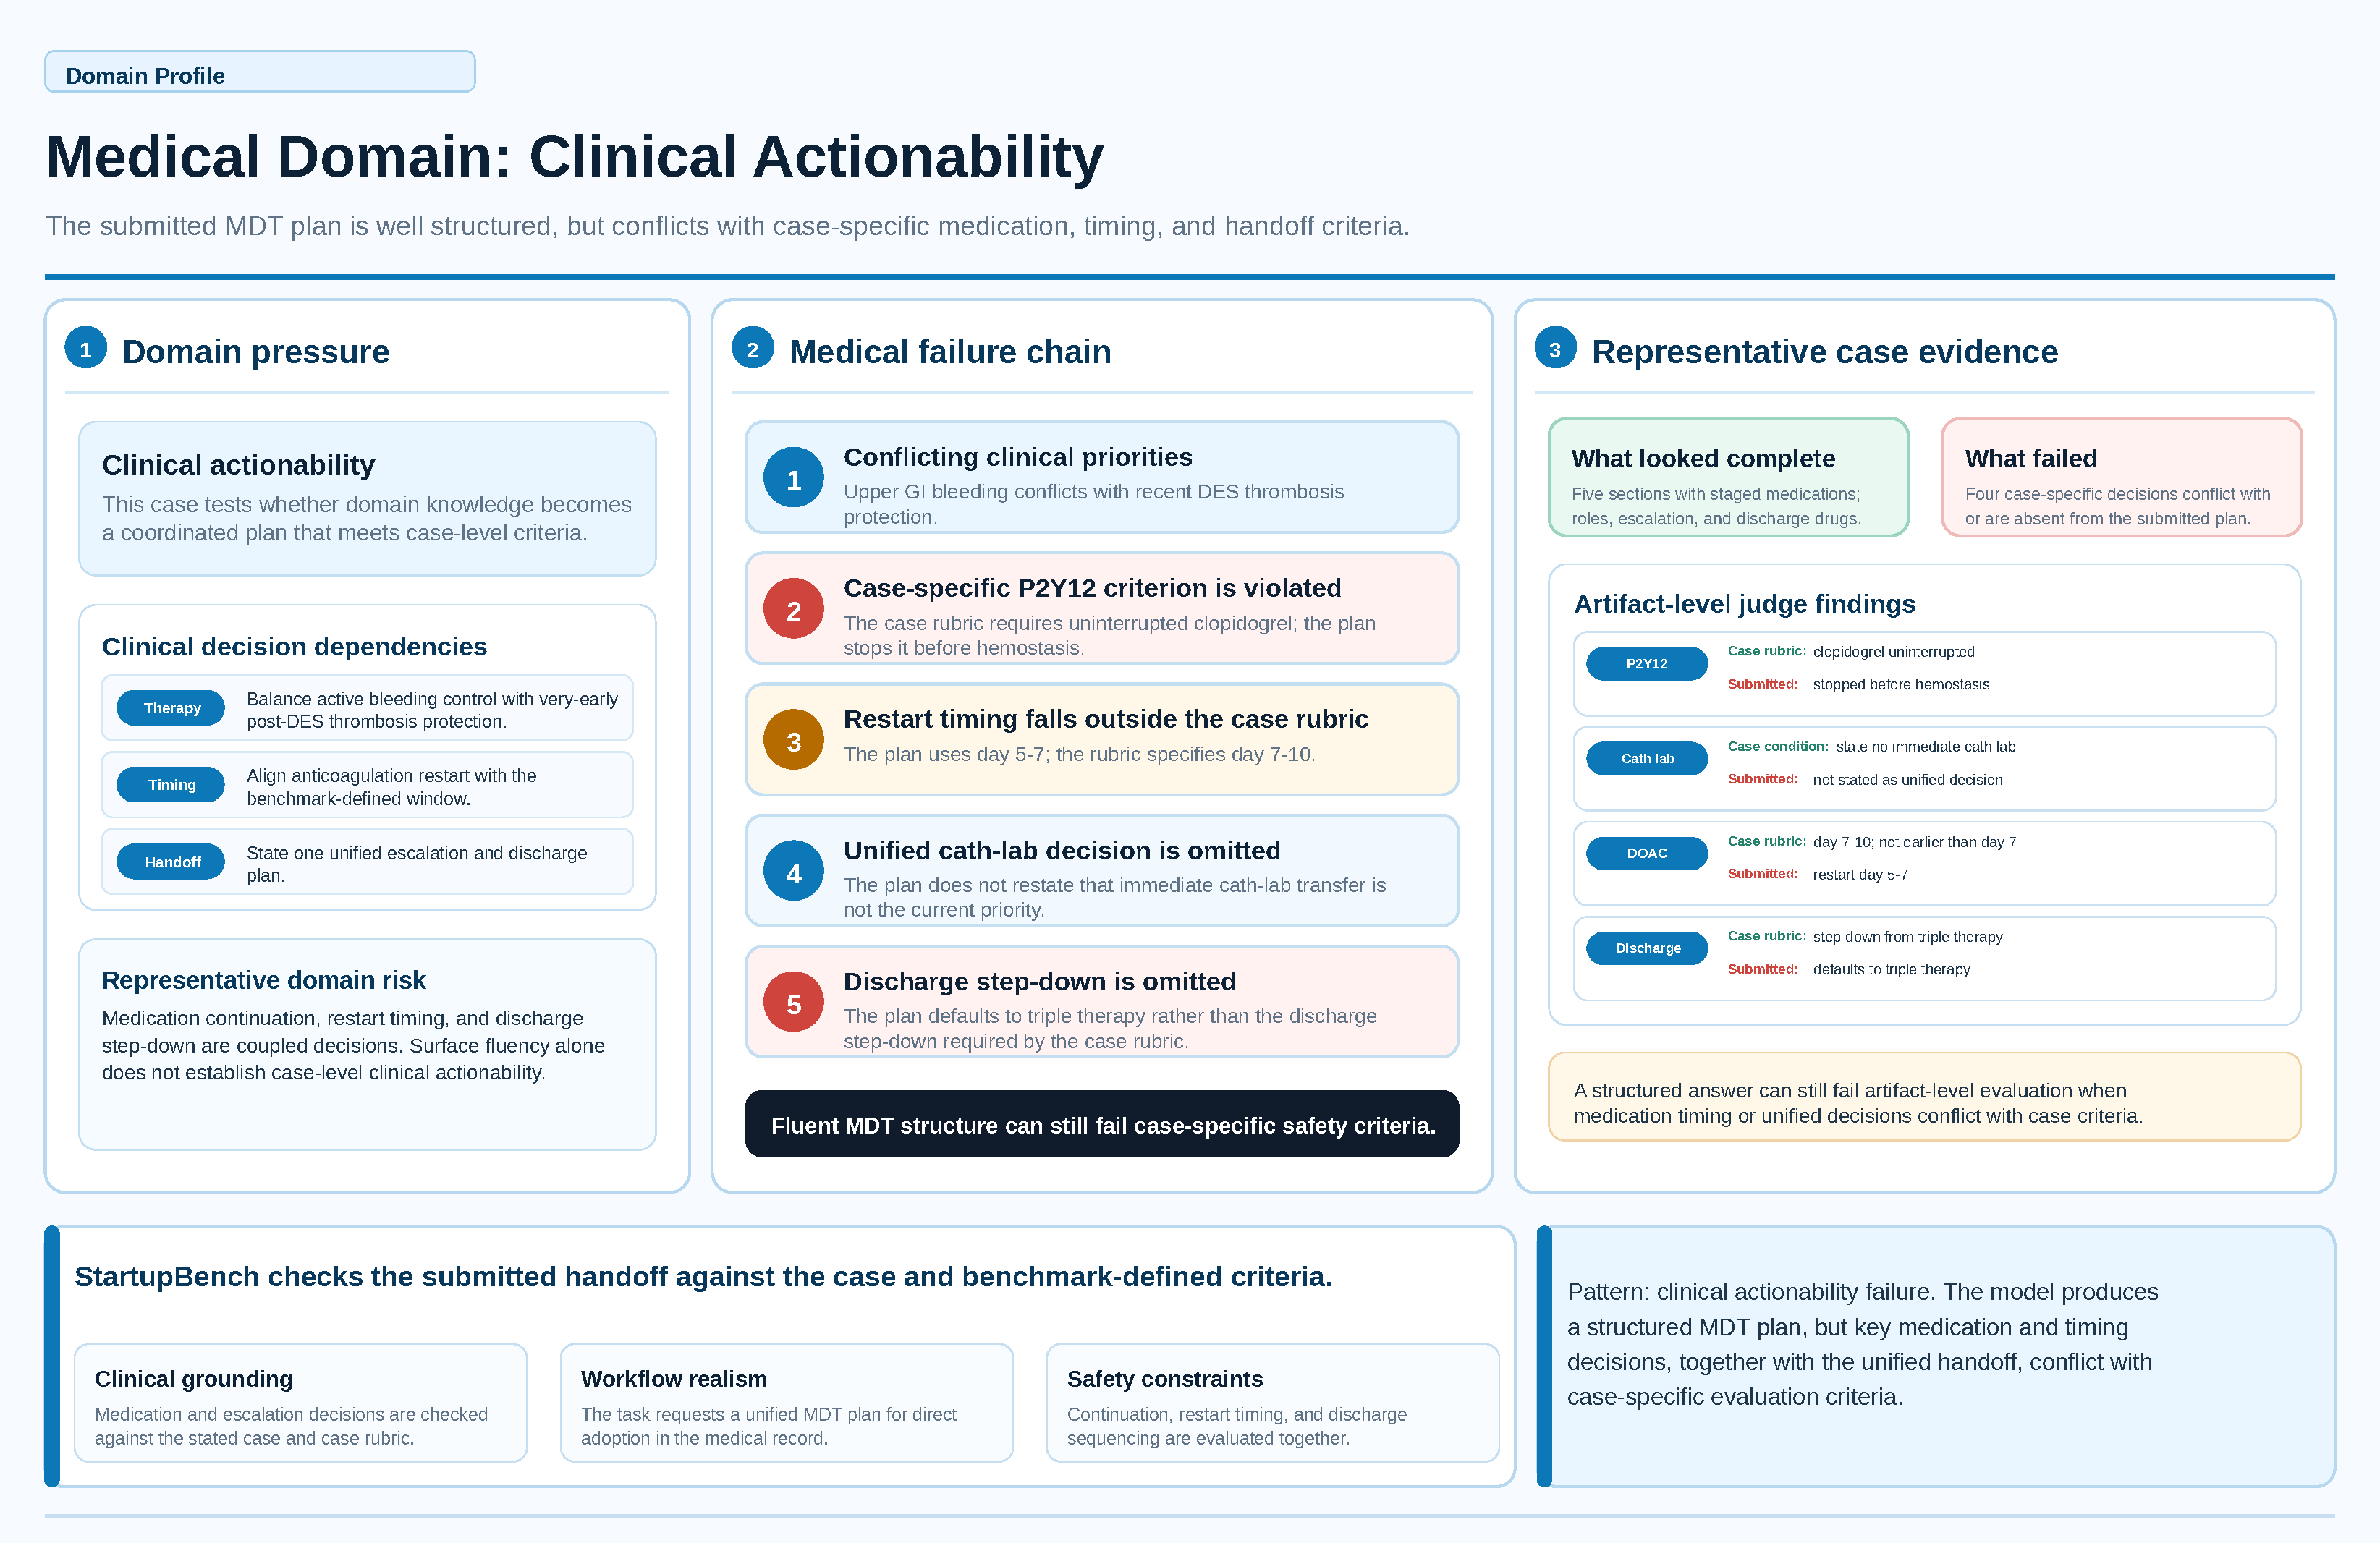
\includegraphics[width=0.99\textwidth]{figures/figure7_medical_clinical_actionability.pdf}
    \caption{由领域特定临床可操作性不足导致的一个代表性失败案例。}
    \label{fig:domain-specify}
\end{figure*}
